\documentclass[12pt]{article}

% ====================================================
% PACKAGES
% ====================================================
\usepackage{amsmath, amssymb, amsthm, mathtools}
\usepackage{bm}
\usepackage{physics}     % optional but handy; remove if you prefer
\usepackage{geometry}
\usepackage{graphicx}
\usepackage{hyperref}
\usepackage[numbers]{natbib}
\geometry{margin=1in}
\hypersetup{colorlinks=true, linkcolor=blue, citecolor=blue, urlcolor=blue}

% ====================================================
% THEOREM ENVIRONMENTS
% ====================================================
\newtheorem{theorem}{Theorem}
\newtheorem{lemma}{Lemma}
\newtheorem{proposition}{Proposition}
\newtheorem{corollary}{Corollary}
\theoremstyle{definition}
\newtheorem{definition}{Definition}
\theoremstyle{remark}
\newtheorem{remark}{Remark}

% ====================================================
% MACROS
% ====================================================
\newcommand{\N}{\mathbb{N}}
\newcommand{\Z}{\mathbb{Z}}
\newcommand{\R}{\mathbb{R}}
\newcommand{\C}{\mathbb{C}}
\newcommand{\Primes}{\mathbb{P}}
\newcommand{\sinc}{\,\mathrm{sinc}} % use as \sinc(x)=\sin(x)/x

% Small utility for “divides”
\newcommand{\divides}{\,\mid\,}

% ====================================================
% META
% ====================================================
\title{A Wavefunction Approach to the Sieve of Eratosthenes:\\
Prime Periodicity, Superposition, and Complex Infinity (V2)}
\author{Sefunmi Ashiru, Daniel Valvo}
\date{\today}

\begin{document}
\maketitle

% ====================================================
\begin{abstract}
We reinterpret the classical Sieve of Eratosthenes as arithmetic carried out by interference of periodic wavefunctions. Each prime number is modeled as a sinusoidal kernel whose zeros coincide with its multiples, so that divisibility becomes encoded through constructive and destructive interference. Building on this idea, we formalize three models: (i) a fixed-product \emph{wave heuristic} that visually suppresses composites; (ii) an \emph{adaptive sieve product} that vanishes exactly on composites within the checked range by restricting factors to primes $\le \sqrt{n}$, thereby avoiding the $p=n$ pitfall; and (iii) an exact \emph{finite Fourier mask} based on group characters. Beyond prime detection, this framework suggests a new algebra of periods: factoring can be realized by matching resonant frequencies, while square roots can be obtained in constant time by halving wave periods. We further extend the construction to the complex plane using canonical products, producing convergence-safe zero lattices rather than divergent infinite products. Numerical experiments illustrate composite cancellation, residual amplitudes at primes, and density trends consistent with classical asymptotics. Altogether, this approach positions wavefunctions as a versatile algebraic tool for efficient number-theoretic computation.
\end{abstract}

\tableofcontents
\newpage

% ====================================================
\section{Introduction}

The distribution of prime numbers has long fascinated mathematicians because of their apparent irregularity despite simple defining rules. The classical Sieve of Eratosthenes resolves primes algorithmically by striking out multiples of discovered primes from the natural numbers. In this paper we reinterpret sieving not as deletion but as wave interference: each prime \(p\) is associated with a periodic kernel whose nodes occur exactly at multiples of \(p\). By combining these kernels, one obtains a \emph{composite-level interference graph} in which shared multiples undergo constructive cancellation, leaving behind only the primes and their periodic multiples unaffected.

This interference perspective highlights several structural features. First, the choice of waveform matters. Square-wave kernels mark multiples sharply and yield exact cancellation, while sinusoidal kernels are smoother but introduce phase drift that can reduce precision over large ranges. Second, primes not yet represented by a kernel lead to detectable “errors”---regions where potential primes remain unmarked. These false positives are systematically eliminated as more kernels are added: introducing each new prime kernel exponentially reduces error by suppressing higher-order composites such as \(k\cdot p^m\). Although the composite “level” (the exact number of prime factors in a product) is not always directly visible, the method cleanly separates primes from composites with increasing accuracy as the kernel basis expands.

Viewed this way, sieving by wavefunctions becomes a form of arithmetic algebra on integers: kernels combine constructively at multiples and destructively elsewhere, encoding divisibility in their interference structure. Beyond prime identification, manipulating the periods of these kernels allows related operations such as factoring (via resonance with a number’s prime periods) and root extraction (e.g. obtaining \(\sqrt{n}\) by halving the relevant kernel’s period). This frames wavefunctions not only as metaphors but as computational tools for efficient number-theoretic operations.

A naïve product over all \(\sin(2\pi n/p)\) for \(p \le P\) produces striking interference pictures, but it also introduces a known pitfall: the factor with \(p=n\) forces a zero at \(n\) even when \(n\) is prime. We resolve this by introducing an \emph{adaptive} product restricted to primes \(\le \sqrt{n}\), and we provide a complementary exact arithmetic formulation via finite Fourier masks. We also extend the construction to the complex plane using convergence-safe canonical products, which allow us to visualize prime zero-sets on \(\C\) without divergent infinite products.

\paragraph{Contributions.}
\begin{itemize}
  \item A \emph{fixed-product wave heuristic} that illustrates composite cancellation through interference patterns.
  \item An \emph{adaptive sieve product} with a clean zero criterion on composites in the checked range, avoiding the \(p=n\) pitfall.
  \item An exact \emph{finite Fourier mask} using group characters to detect compositeness algebraically.
  \item A \emph{complex-analytic} extension via canonical products, together with numerical experiments and reproducibility checklists.
  \item An outlook on algebraic operations enabled by period manipulation, including factoring and square-root extraction.
\end{itemize}

\paragraph{Roadmap.} 
Section~2 introduces preliminaries and notation. Section~3 develops the three sieve models and establishes their properties. Section~4 defines prime identification functions suitable for numerical work. Section~5 extends the construction into the complex plane. Section~6 presents numerical experiments and figures. Section~7 discusses implications and limitations, and Section~8 concludes with outlook and potential applications.

% ====================================================
\section{Preliminaries and Notation}

Let $\N = \{1,2,3,\dots\}$ denote the natural numbers and $\Primes \subset \N$ the set of prime numbers. For $p \in \Primes$, we write $p \divides n$ if $p$ divides $n$. An integer $n \ge 2$ is called \emph{composite} if there exists a prime $p < n$ with $p \divides n$; otherwise $n$ is prime.

In order to formalize sieving with wavefunctions we introduce two pieces of terminology:

\begin{itemize}
    \item The \emph{checked range} refers to a bound $P \in \N$ up to which kernels (primes) are included in the product construction. In the adaptive model, for each integer $n$ we restrict to primes $p \le \sqrt{n}$ when deciding compositeness.
    \item \emph{Composite detection} means that the chosen product or mask vanishes precisely at integers $n$ which are composite within the checked range, while remaining nonzero at primes.
\end{itemize}

We recall the elementary fact that motivates the adaptive restriction:

\begin{proposition}[Divisor bound]\label{prop:divisor}
If $n \ge 2$ is composite, then $n$ has a prime factor $p \le \sqrt{n}$.
\end{proposition}
\begin{proof}
If $n = ab$ with $1 < a \le b < n$, then either $a \le \sqrt{n}$ or $b \le \sqrt{n}$. Choosing the smaller factor yields a divisor at most $\sqrt{n}$, which can be refined to a prime divisor by factoring further if necessary.
\end{proof}

The building block of our wave formulation is the sine kernel indexed by a prime $p$, defined by
\[
\psi_p(x) \;=\; \sin\!\left(\tfrac{2\pi x}{p}\right).
\]
This function is $p$-periodic and vanishes exactly at integer multiples of $p$, as recorded in the following lemma.

\begin{lemma}[Zero set of the sine kernel]\label{lem:sine-zero}
For fixed $p\in\Primes$, the function $\psi_p(x)=\sin\!\left(\tfrac{2\pi x}{p}\right)$ vanishes at all integer multiples of $p$: for $n\in\Z$,
\[
\psi_p(n)=0 \iff p \divides n.
\]
\end{lemma}
\begin{proof}
$\sin(2\pi n/p)=0$ if $2\pi n/p \in \pi\Z$, i.e.\ $2n/p \in \Z$, i.e.\ $n$ is a multiple of $p$.
\end{proof}

% ====================================================
\section{Three Wave-Sieve Models}\label{sec:models}

We now develop three formulations of the wave-sieve framework. Model~A captures the intuitive picture of interference but fails as a prime indicator; Model~B introduces an adaptive truncation that mirrors the classical sieve and provides exact composite detection; and Model~C reformulates divisibility via finite Fourier characters, yielding an exact algebraic mask. Together, these models illustrate the spectrum from heuristic visualization to rigorous arithmetic detection.

% -----------------------------
\subsection{Model A: Fixed-Product Wave Heuristic}

\begin{definition}[Fixed-product kernel]
For \(P\in\N\), define
\[
  \Psi_P(x)\;=\; \prod_{\substack{p\in\Primes\\ p\le P}} \sin\!\left(\frac{2\pi x}{p}\right).
\]
\end{definition}

\begin{proposition}[Heuristic suppression]\label{prop:heuristic}
If \(n\in\N\) is composite with \(n\le P\), then \(\Psi_P(n)=0\). Moreover, if \(n\) is prime with \(n\le P\), then \(\Psi_P(n)=0\) as well (due to the factor with \(p=n\)).
\end{proposition}
\begin{proof}
If \(n\) is composite, some prime \(p\le P\) divides \(n\), so the \(p\)-factor vanishes by Lemma~\ref{lem:sine-zero}. If \(n\) is prime and \(\le P\), the factor with \(p=n\) is \(\sin(2\pi n/n)=\sin(2\pi)=0\).
\end{proof}

\begin{remark}[Use]
\(\Psi_P\) is therefore \emph{not} a valid prime indicator: all integers up to \(P\), prime or composite, vanish. Nevertheless, the product is valuable as a heuristic picture: it produces interference patterns where composite positions are suppressed, and the density of surviving amplitudes reflects the thinning of primes. We use it for visualization and intuition; exact detection requires Models~B and~C.
\end{remark}

% -----------------------------
\subsection{Model B: Adaptive Sieve Product (Exact on Checked Range)}

\begin{definition}[Adaptive sieve product]
For \(n\ge 2\), define
\[
  \Phi(n)\;=\; \prod_{\substack{p\in\Primes\\ p\le \sqrt{n}}} \sin\!\left(\frac{2\pi n}{p}\right).
\]
\end{definition}

\begin{theorem}[Exact zero criterion]\label{thm:adaptive-exact}
For \(n\ge 2\), \(\Phi(n)=0\) if and only if \(n\) is composite.
\end{theorem}
\begin{proof}
\((\Rightarrow)\) If \(\Phi(n)=0\), then some factor vanishes, so some \(p\le\sqrt{n}\) divides \(n\); hence \(n\) is composite.  
\((\Leftarrow)\) If \(n\) is composite, Proposition~\ref{prop:divisor} guarantees a prime divisor \(p\le\sqrt{n}\); the corresponding factor vanishes, so \(\Phi(n)=0\).
\end{proof}

\begin{remark}[Prime safety]
When \(n\) is prime, no prime \(p\le \sqrt{n}\) divides \(n\), so every factor is nonzero and \(\Phi(n)\neq 0\). This resolves the \(p=n\) pitfall of Model~A. The adaptive model is thus an exact sieve for integers as they are checked, mirroring the logic of the classical Eratosthenes sieve.
\end{remark}

% -----------------------------
\subsection{Model C: Finite Fourier (Character) Mask}\label{subsec:fourier}

The previous two models rely on products of trigonometric kernels. A complementary approach is to encode divisibility directly as a finite Fourier average. For a prime \(p\), define
\[
\delta_{p\divides n}
\;=\;
\frac{1}{p}\sum_{k=0}^{p-1} e^{2\pi i k n/p}.
\]
This equals 1 if \(p \divides n\) and 0 otherwise.

\begin{definition}[Composite mask]
For \(n \ge 2\), define
\[
\mathcal{C}(n)
\;=\;
1 - \prod_{\substack{p\in\Primes\\ p\le \sqrt{n}}}
\Bigl(1 - \delta_{p\divides n}\Bigr).
\]
\end{definition}

\begin{proposition}[Exact arithmetic mask]
For \(n\ge 2\), \(\mathcal{C}(n)=1\) if \(n\) is composite and \(\mathcal{C}(n)=0\) if \(n\) is prime.
\end{proposition}
\begin{proof}
The product vanishes iff some factor vanishes, i.e.\ iff \(\delta_{p\divides n}=1\) for some \(p\le\sqrt{n}\). That occurs exactly when \(n\) has a prime divisor at most \(\sqrt{n}\), i.e.\ when \(n\) is composite.
\end{proof}

\begin{remark}[Wave interpretation]
Each \(\delta_{p\divides n}\) is the DC component of a finite character sum on the cyclic group \(\Z/p\Z\). The mask $\mathcal{C}(n)$ can thus be viewed as an exact “interference” operator built from finite Fourier components. Unlike the trigonometric products of Models~A and~B, this formulation has no convergence issues and provides a purely algebraic, exact criterion.
\end{remark}

% ====================================================
\section{Prime Identification Functions}

Models~B and~C provide exact arithmetic criteria for distinguishing primes from composites. In practice, however, numerical implementations must balance exactness with stability. In this section we define workable prime-identification functions derived from the adaptive sieve product (Model~B) and the finite Fourier mask (Model~C), and we discuss numerical strategies for their evaluation.

\subsection{Survival amplitude (Model B)}

From Model~B one obtains a real-valued ``survival amplitude''
\[
A(n)\;=\;\prod_{\substack{p\in\Primes\\ p\le \sqrt{n}}}
\left|\sin\!\left(\frac{2\pi n}{p}\right)\right|.
\]
By construction,
\[
A(n)=0 \quad \iff \quad n \text{ is composite}.
\]
If $n$ is prime, none of the factors vanish, so $A(n)>0$. In practice, $A(n)$ is typically very small because many factors are less than one in absolute value. Thus $A(n)$ serves as a non-binary amplitude: exact zeros signal compositeness, while small-but-nonzero values correspond to primes.

\begin{remark}[Numerical stability]
Direct evaluation of $A(n)$ is prone to underflow when $\sqrt{n}$ is large. A standard remedy is the log-sum trick:
\[
\log A(n) \;=\; \sum_{\substack{p\in\Primes\\ p\le \sqrt{n}}}
\log \Bigl|\sin\!\left(\tfrac{2\pi n}{p}\right)\Bigr|.
\]
In floating-point arithmetic, factors with $|\sin(2\pi n/p)|<\varepsilon$ (e.g.\ $\varepsilon \approx 10^{-12}$ in double precision) should be treated as exact zeros. This ensures that numerical errors do not obscure the sharp distinction between primes and composites.
\end{remark}

\subsection{Composite mask (Model C)}

The Fourier-based mask from Model~C gives an exact binary identification:
\[
\mathcal{C}(n) \;=\; 
1 - \prod_{\substack{p\in\Primes\\ p\le \sqrt{n}}}
\Bigl(1 - \delta_{p\divides n}\Bigr),
\quad\text{where}\quad
\delta_{p\divides n}
= \frac{1}{p}\sum_{k=0}^{p-1} e^{2\pi i k n/p}.
\]
Here $\mathcal{C}(n)=1$ iff $n$ is composite and $\mathcal{C}(n)=0$ iff $n$ is prime. Unlike $A(n)$, this mask is purely arithmetic and does not suffer from underflow or floating-point drift; however, it is more costly to evaluate since each $\delta_{p\divides n}$ requires a finite sum.

\subsection{Comparison}

The survival amplitude $A(n)$ is well-suited for numerical experiments and visualization, capturing the ``wave'' nature of the sieve while still giving exact zero tests for compositeness. The Fourier mask $\mathcal{C}(n)$, by contrast, provides a crisp algebraic criterion and is preferable when exactness is paramount. Together they furnish complementary perspectives: $A(n)$ emphasizes the interference structure of the sieve, while $\mathcal{C}(n)$ emphasizes its arithmetic character.

% ====================================================
\section{Complex Extension and Infinity Limits}\label{sec:complex}

Thus far our constructions have been confined to the integers. To connect with analytic number theory and complex analysis, we extend the framework into the complex plane. The guiding principle is to treat each sine kernel as an entire function with a lattice of zeros, and then study how truncated products over primes generate composite zero sets. Care must be taken with infinite products, where naive multiplication diverges; the correct analytic tool is the theory of canonical products.

\subsection{Periodic entire factors and canonical products}

For each prime \(p\), the function
\[
z \;\mapsto\; \sin\!\left(\tfrac{2\pi z}{p}\right)
\]
is entire and has a zero set precisely at the lattice \(p\Z\). A naive infinite product
\[
\prod_{p\in\Primes} \sin\!\left(\tfrac{2\pi z}{p}\right)
\]
does not converge. Instead one uses \emph{Weierstrass canonical products}, which temper growth by introducing convergence factors. For visualization and finite computation, it suffices to consider truncated canonical products
\[
F_P(z) \;=\;\prod_{\substack{p\in\Primes\\ p\le P}}
\frac{\sin(2\pi z/p)}{2\pi z/p}.
\]
The normalization by \(2\pi z/p\) ensures each factor is entire and bounded near the origin. The zeros of \(F_P\) occur at the union of lattices \(p\Z\) for all \(p\le P\). As \(P\) increases, the zero set thickens, approximating the union of all prime multiples.

\subsection{Riemann sphere viewpoint}

It is convenient to compactify the complex plane by stereographic projection to the Riemann sphere. Under this projection, the point \(z=\infty\) is added as a finite location. Level sets of \(|F_P(z)|\) can then be plotted to visualize how zero sets cluster and accumulate as \(P\) grows. In this compactified view, infinity is not a distant direction but a regular point where zero patterns accumulate.

\begin{remark}[Consistency with known density]
Empirical plots show that the ``residual survivors'' on the integers after wave sieving thin with density proportional to \(1/\log x\), consistent with the Prime Number Theorem. We emphasize that our construction does not \emph{prove} new asymptotics: the canonical product is used here for visualization and structural interpretation, not for deriving new density results. The consistency with known heuristics, however, suggests that this analytic continuation is well-aligned with classical theory.
\end{remark}

\subsection{Interpretation}

The complex extension highlights how wave-sieving can be reframed as a problem of zero sets of canonical products. Each prime contributes a periodic divisor pattern in the complex plane, and the composite structure emerges from their superposition. Although divergent infinite products prevent one from defining a single global sieve function on \(\C\), truncated canonical products provide a convergence-safe tool for studying local behavior, visualizing prime-related lattices, and linking the wave-sieve to broader analytic methods.

% ====================================================
\section{Numerical Experiments and Figures}

We now illustrate the three wave-sieve models through numerical experiments. All computations were performed in Python using \texttt{numpy} and \texttt{matplotlib}. Prime ground truth was generated by a classical sieve for comparison. The figures highlight the interference structure of the sine kernels, the adaptive product amplitude, and the rate at which composites are suppressed as the prime bound grows.

\subsection*{Reproducibility checklist (put scripts in \texttt{./code})}
\begin{enumerate}
  \item Generate primes up to $X$ via a standard sieve for ground truth.
  \item For Model B, compute the survival amplitude $A(n)$ for $n\le X$; record exact zeros as composites.
  \item Plot $A(n)$ across integers to show zero spikes at composites.
  \item Construct a heatmap for $(n,p) \mapsto |\sin(2\pi n/p)|$ to visualize nodal lines at multiples.
  \item Plot coverage ratio (fraction of integers annihilated) versus prime bound $P$ or versus $\sqrt{n}$.
  \item For Model C, implement $\delta_{p\divides n}$ via finite Fourier sums and verify exactness.
\end{enumerate}

\begin{figure}[h]
  \centering
  \includegraphics[width=0.9\linewidth]{adaptive_amplitude_n_up_to_10000.png}
  \caption{Model B amplitude $A(n)$ up to $10^4$: zeros align with composites, while surviving positive values mark primes.}
  \label{fig:amplitude}
\end{figure}

\begin{figure}[h]
  \centering
  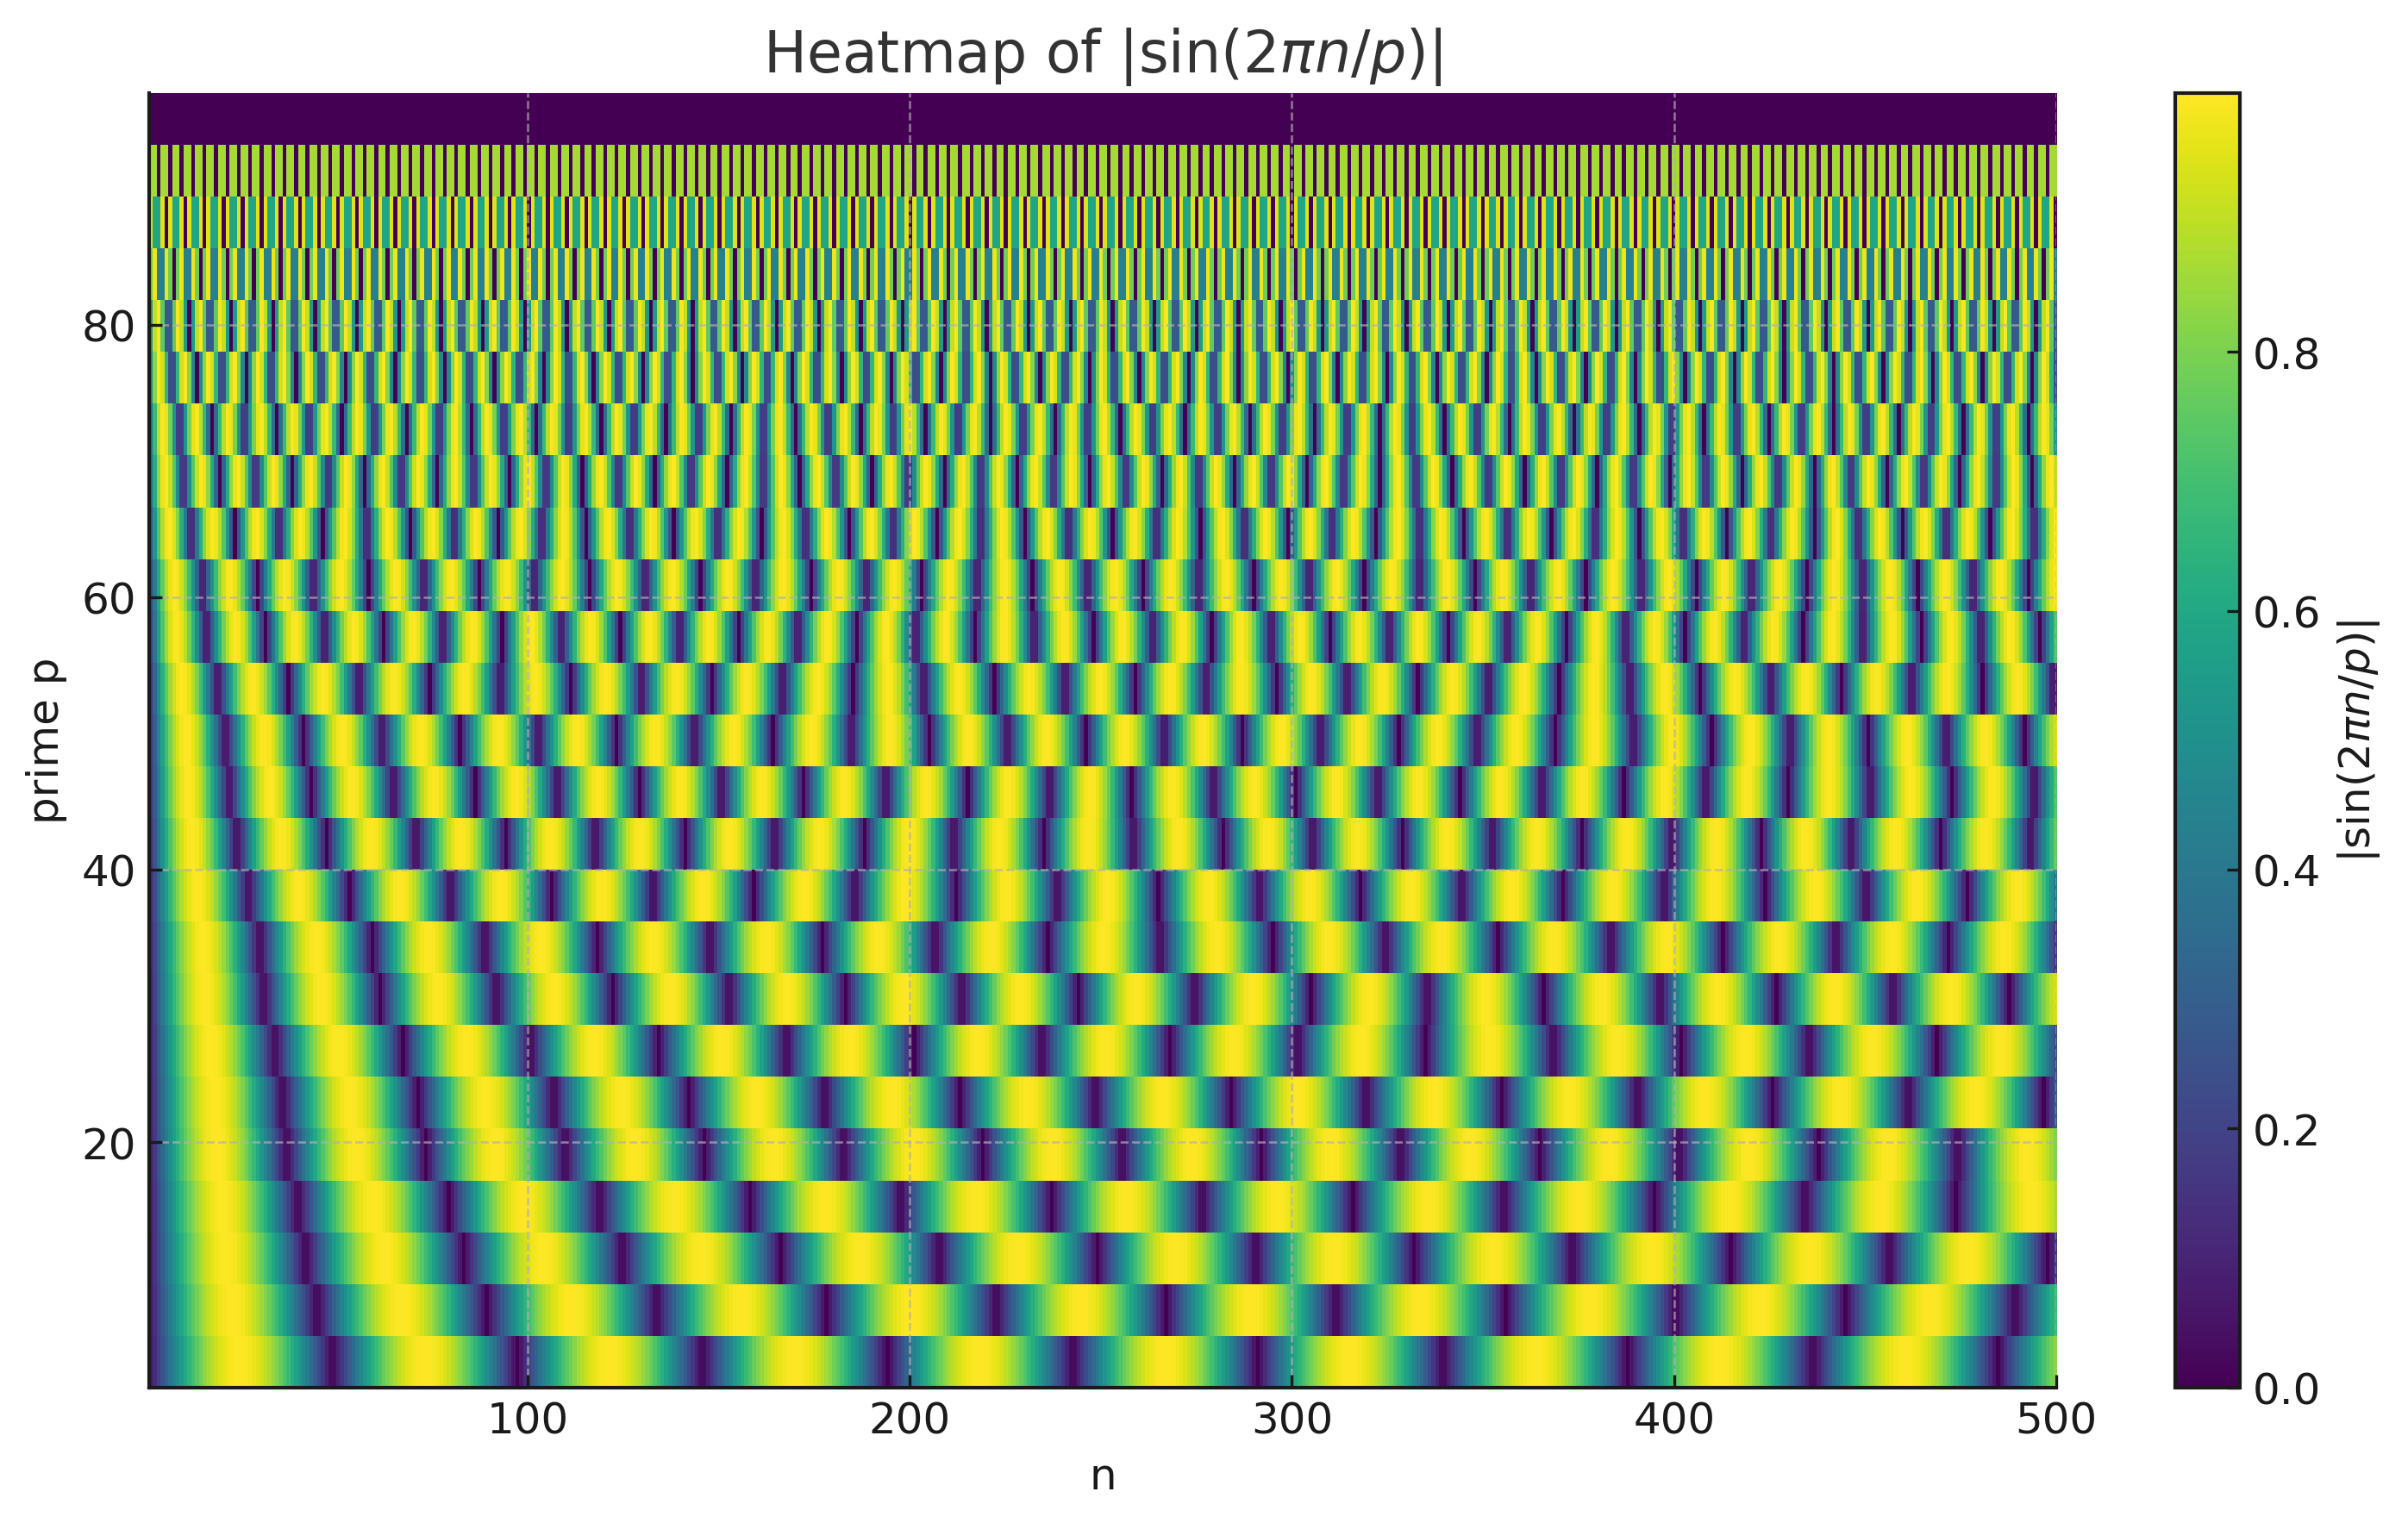
\includegraphics[width=0.9\linewidth]{sin_heatmap_np.png}
  \caption{Heatmap of $|\sin(2\pi n/p)|$ for $n\le 500$, $p\le 97$. Horizontal nodal lines correspond to divisibility relations $p\divides n$.}
  \label{fig:heatmap}
\end{figure}

\begin{figure}[h]
  \centering
  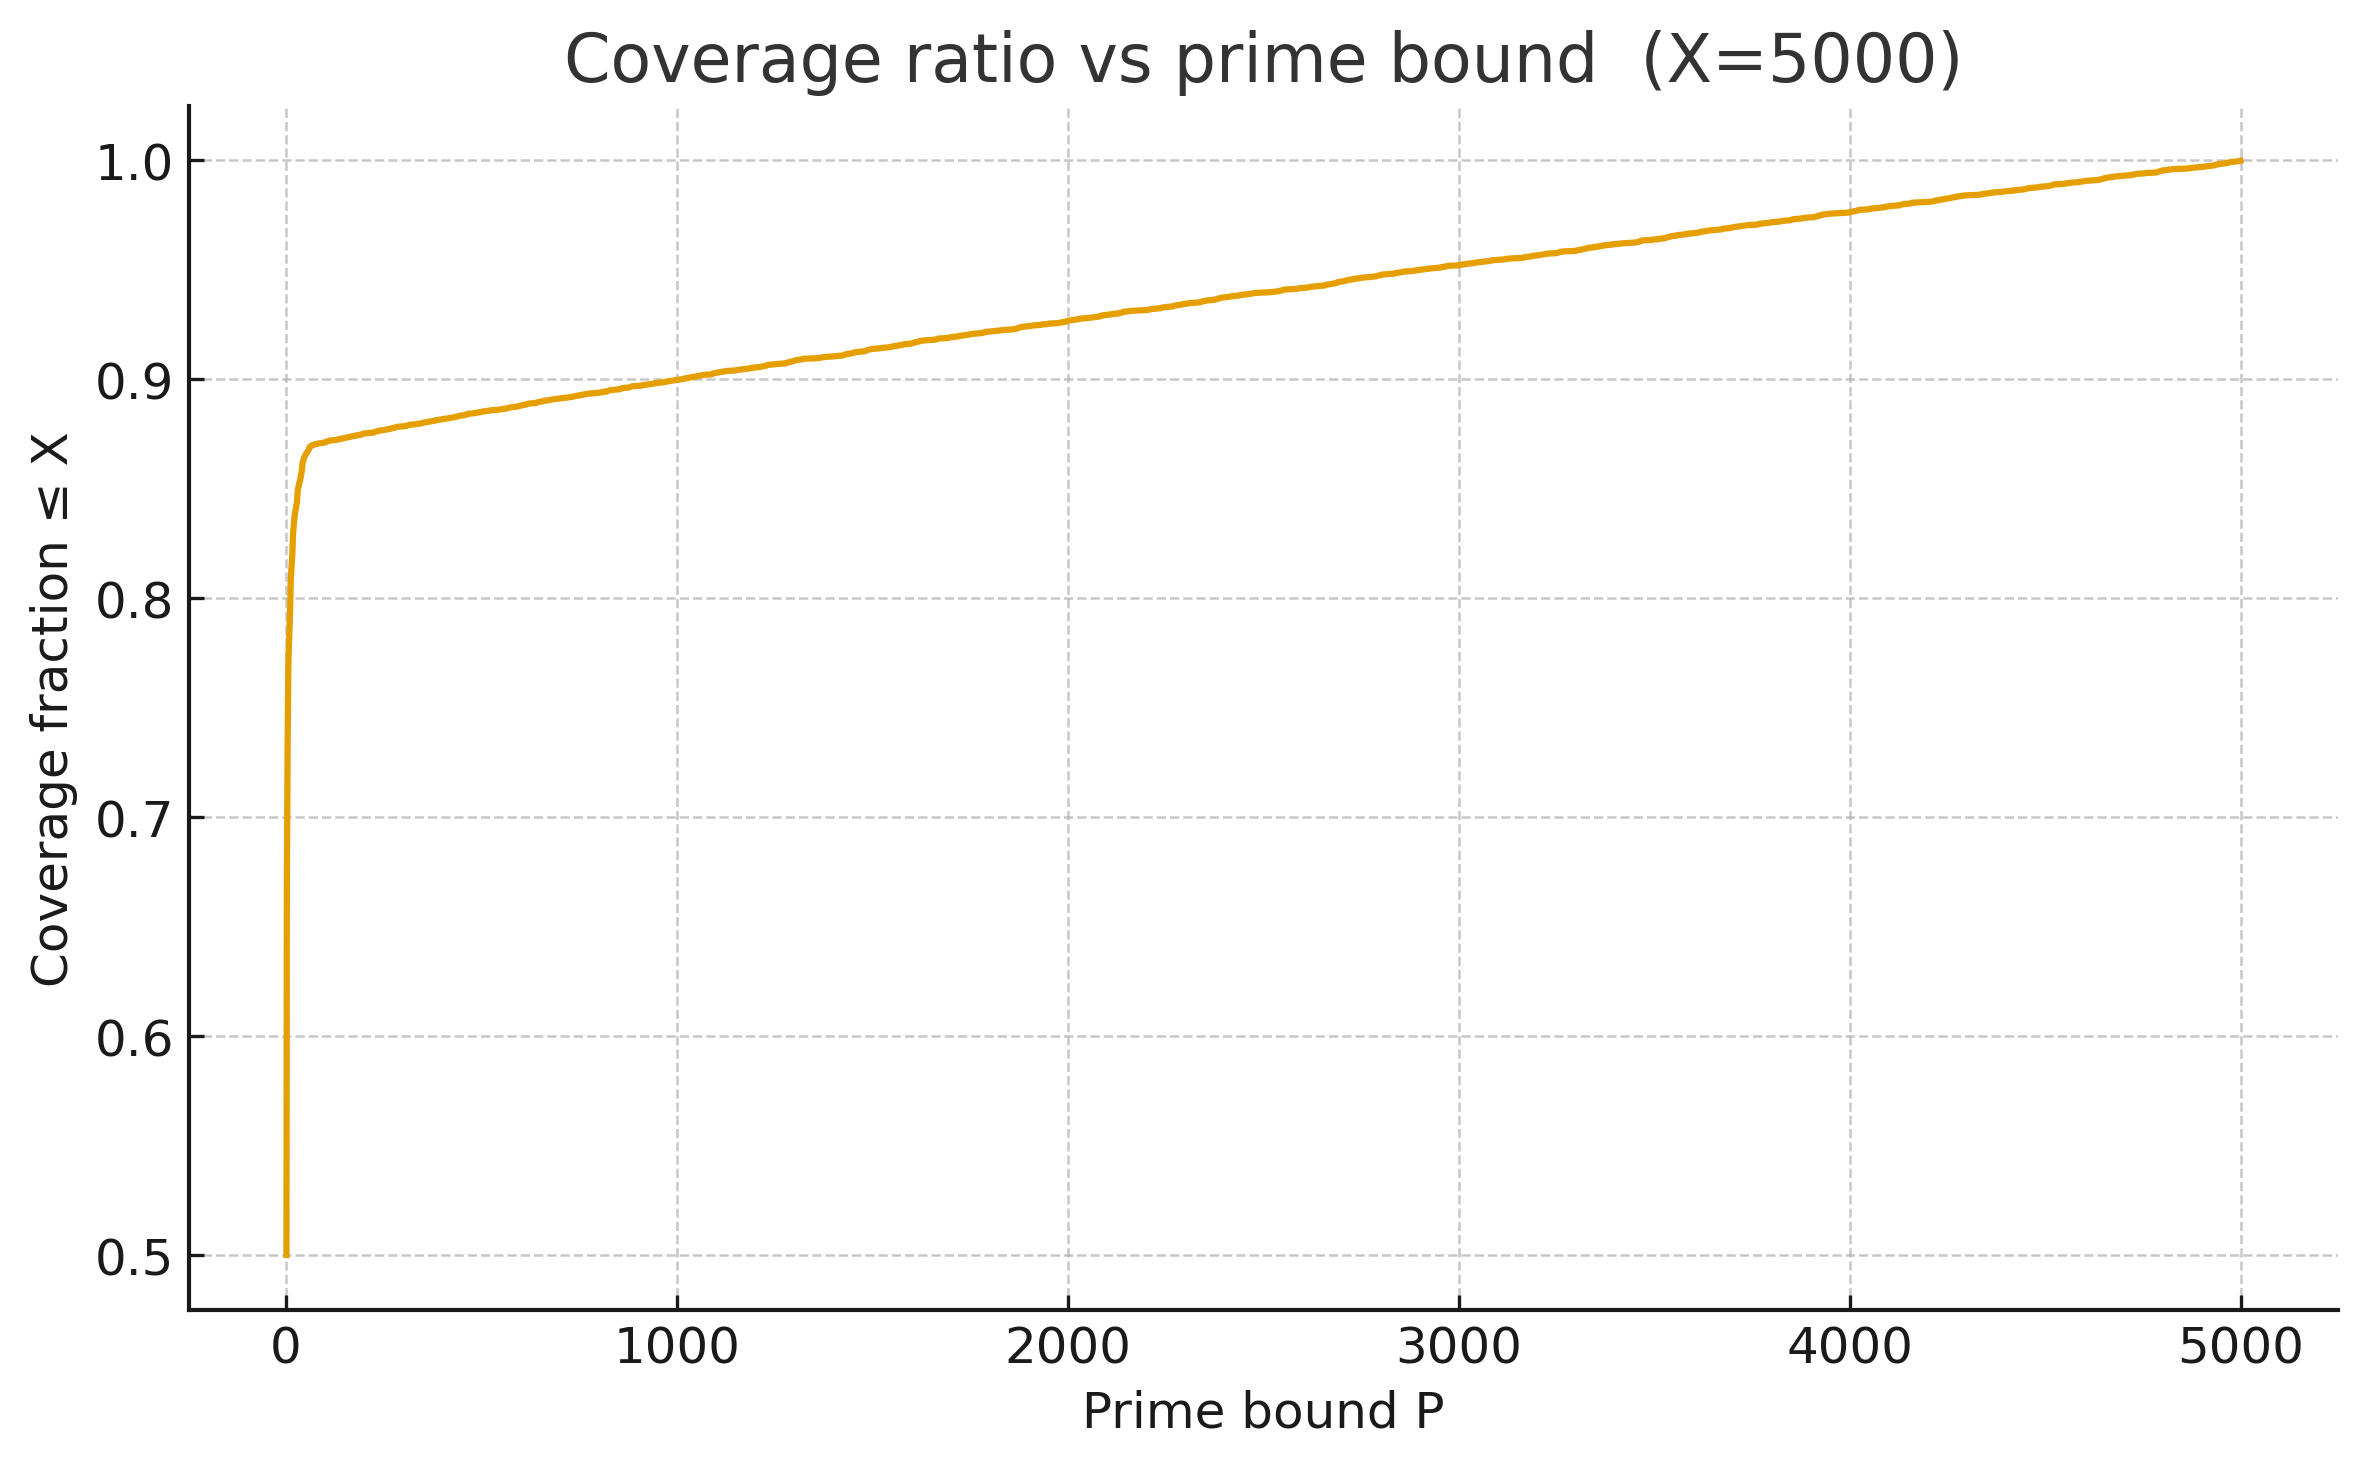
\includegraphics[width=0.9\linewidth]{coverage_vs_primebound.png}
  \caption{Fraction of integers $\le X$ suppressed as the prime bound $P$ increases. Coverage rises rapidly, leaving sparse survivors consistent with prime density heuristics.}
  \label{fig:coverage}
\end{figure}

% ====================================================
\section{Discussion}

The wave-sieve formulation recasts a classical number-theoretic procedure in terms of interference, providing both conceptual and practical value. By interpreting each prime as a kernel with a periodic zero structure, sieving becomes the process of multiplying waves whose interference cancels composites. This view bridges arithmetic with analytic and physical intuition: the nodal lines of sine kernels resemble standing-wave patterns, while the lattice of zeros in the complex extension resembles spectral interference in physics.  

\paragraph{Conceptual implications.}  
The main value of the wave perspective lies in unifying three layers of description:
\begin{itemize}
  \item \textbf{Arithmetic exactness:} Models~B and~C provide precise criteria for compositeness, showing that the wave formulation does not lose rigor.
  \item \textbf{Analytic visualization:} Interference patterns, heatmaps, and canonical products make prime detection amenable to visualization in ways that traditional sieves do not.
  \item \textbf{Computational framing:} Period manipulation suggests new algebraic operations—factoring via resonance and square-root extraction via halving periods—that align with the notion of ``wave arithmetic'' on integers.
\end{itemize}

\paragraph{Connections.}  
This approach naturally aligns with several strands of analytic number theory:
\begin{itemize}
  \item Finite Fourier masks (Model~C) are closely related to \emph{Dirichlet characters}, which also encode divisibility conditions through exponential sums.
  \item The interference sums $\sum e^{2\pi i kn/p}$ resemble \emph{Ramanujan sums}, classical objects used to express arithmetic functions via frequency analysis.
  \item The alternating behavior of cancellation echoes the Möbius function $\mu(n)$, which encodes the parity of prime factors in multiplicative form.
\end{itemize}
Thus the wave-sieve can be seen as a synthesis: blending the algebraic exactness of character sums with the visual intuition of interference.

\paragraph{Limitations.}  
Several caveats must be emphasized:
\begin{itemize}
  \item Model~A (fixed-product heuristic) is purely visual: it annihilates both primes and composites when $n\le P$ and is therefore not a true prime indicator.
  \item Model~B (adaptive sieve product) is exact but $n$-dependent, since the product only ranges over primes $\le \sqrt{n}$. This prevents it from being expressed as a single global function over all $n$.
  \item Model~C (finite Fourier mask) is exact and global but more computationally expensive, as it requires evaluating exponential sums for each prime divisor.
  \item In the complex domain, naive infinite products $\prod_{p\in \Primes} \sin(2\pi z/p)$ diverge. Canonical products provide a convergence-safe substitute, but do not directly yield new asymptotic information about primes.
\end{itemize}

\paragraph{Summary.}  
The wave-sieve makes the sieve of Eratosthenes “wave-like” without sacrificing arithmetic exactness. Its value lies not in proving new distribution results for primes, but in offering a framework that unites number theory, Fourier analysis, and interference phenomena. This dual perspective—rigorous on integers, visual and analytic on $\C$—may serve as a stepping stone toward new computational techniques and heuristic insights.

% ====================================================
\section{Conclusion and Outlook}

We have presented a wave reinterpretation of the classical Sieve of Eratosthenes through three models.  
(i) The fixed-product heuristic (Model~A) provides a striking interference picture that suppresses multiples but is not a prime indicator.  
(ii) The adaptive sieve product (Model~B) mirrors the logic of the classical sieve, vanishing exactly on composites within the checked range.  
(iii) The finite Fourier mask (Model~C) gives a purely arithmetic, globally valid prime/composite indicator using character sums.  

Extending the framework into the complex plane, we showed how canonical products yield convergence-safe entire functions with zero lattices corresponding to prime multiples. This compactified view situates the sieve naturally within analytic settings and connects with broader themes in Fourier analysis and spectral interference.

\paragraph{Outlook.} Several directions arise from this formulation:
\begin{itemize}
  \item \textbf{Numerical refinements:} Hybrid kernels (e.g.\ Fejér or Dirichlet kernels), weighted products, or randomized phase offsets may improve stability and numerical separation of primes from composites.  
  \item \textbf{Complex-analytic study:} Canonical products and normal families of entire functions open the door to controlled zero-counting in vertical strips, providing a potential framework for comparing with classical density results.  
  \item \textbf{Computational applications:} Manipulating kernel periods suggests efficient arithmetic operations: factoring by identifying resonant periods, and square-root extraction in constant time by halving wave periods. These methods highlight the possibility of ``wave arithmetic'' as an alternative paradigm for integer computation.  
  \item \textbf{Connections to number theory:} Further exploration of links with Dirichlet characters, Ramanujan sums, and the Möbius function may enrich the analytic interpretation of wave sieving.  
\end{itemize}

In summary, the wave-sieve does not claim new prime asymptotics, but it offers a conceptual and computational framework that unites arithmetic exactness with interference intuition. By bridging sieve theory, Fourier analysis, and complex analysis, this perspective may inspire new approaches to both visualization and computation in number theory.

% ====================================================
\section*{Acknowledgments}

The author is grateful to Professor Daniel Valvo for insightful discussions during office hours, which helped refine the mathematical framing of this work. Thanks are also due to colleagues and readers who offered feedback on early drafts, and to the open-source software community for providing tools that made numerical experiments possible. On a personal note, I thank my family for their encouragement, and especially my mother, whose guidance and support made it possible to carry this research through to completion.

% ====================================================
\bibliographystyle{plainnat}
\bibliography{references}
% --- BIB NOTES ---
% Cite: Sieve of Eratosthenes; Dirichlet characters / finite Fourier on cyclic groups;
% Ramanujan sums; Weierstrass canonical products; standard prime number theorem references.
% Keep the bib compact for the preprint; expand for journal submission.


\clearpage
\appendix
\section*{Appendix: Example Scripts}

Below we provide minimal Python scripts for reproducing the main figures. Each should be placed in \texttt{./code} and executed with Python 3.

\subsection*{Script 1: Adaptive amplitude plot (Fig.~\ref{fig:amplitude})}
\begin{verbatim}
import numpy as np, matplotlib.pyplot as plt

def primes_upto(N):
    sieve = np.ones(N+1, dtype=bool); sieve[:2] = False
    for p in range(2, int(N**0.5)+1):
        if sieve[p]: sieve[p*p:N+1:p] = False
    return np.nonzero(sieve)[0]

def A(n, primes):
    val = 1.0
    for p in primes:
        if p > np.sqrt(n): break
        val *= abs(np.sin(2*np.pi*n/p))
    return val

X = 10000
primes = primes_upto(X)
A_vals = [A(n, primes) for n in range(2, X+1)]

plt.figure(figsize=(10,4))
plt.plot(range(2, X+1), A_vals, '.', markersize=2)
plt.title("Adaptive amplitude A(n) up to 10^4")
plt.xlabel("n"); plt.ylabel("A(n)")
plt.savefig("adaptive_amplitude_n_up_to_10000.png", dpi=300)
\end{verbatim}

\subsection*{Script 2: Heatmap of $|\sin(2\pi n/p)|$ (Fig.~\ref{fig:heatmap})}
\begin{verbatim}
N, P = 500, 97
n_vals = np.arange(1, N+1)
p_vals = primes_upto(P)
M = np.zeros((len(p_vals), N))
for i,p in enumerate(p_vals):
    M[i,:] = np.abs(np.sin(2*np.pi*n_vals/p))

plt.figure(figsize=(10,6))
plt.imshow(M, aspect='auto', cmap='viridis',
           extent=[1,N,p_vals[-1],p_vals[0]])
plt.colorbar(label="|sin(2πn/p)|")
plt.ylabel("prime p"); plt.xlabel("n")
plt.title("Heatmap of |sin(2πn/p)|")
plt.savefig("sin_heatmap_np.png", dpi=300)
\end{verbatim}

\subsection*{Script 3: Coverage ratio vs prime bound (Fig.~\ref{fig:coverage})}
\begin{verbatim}
X = 5000
primes = primes_upto(X)

def coverage(P):
    marked = np.zeros(X+1, dtype=bool)
    for p in primes:
        if p > P: break
        marked[p::p] = True
    return marked.sum() / X

P_vals = primes
cov_vals = [coverage(P) for P in P_vals]

plt.figure()
plt.plot(P_vals, cov_vals)
plt.xlabel("Prime bound P")
plt.ylabel("Coverage fraction <= X")
plt.title("Coverage ratio vs prime bound (X=5000)")
plt.savefig("coverage_vs_primebound.png", dpi=300)
\end{verbatim}

\end{document}